\chapter{Software for crowd guidance systems based on direct communication  }
\label{sec:crownet}

In this chapter I develop the scientific software \textit{CrowNet} (\underline{Crow}ds in \underline{Net}works) that I use for the investigation of my research questions in Chapter~\ref{sec:investigation}. 
The chapter is structured as follows: First I give an introduction into the simulation framework \textit{CrowNet}. I define its scope, requirements, quality measures and I present the software architecture. Since \textit{CrowNet} has been developed in collaboration with other researchers (see Appendix~\ref{sec:collaboration}), I address which parts of the software were developed by me and which parts of the software I use but which were developed by other researchers. I then go into the development of the individual modules. Some modules are based on existing simulation frameworks known from the previous chapter. I show how these frameworks have been extended for their integration into \textit{CrowNet}. Other modules provide novel models or procedures for which no software was available. I will present the respective concepts and their implementations. In this, I will focus on functionalities and features that are mandatory for the investigation of my research questions. A description of all available features of the \textit{CrowNet} framework can be found in the software documentation. At the end of the chapter I give an overview of the functionalities that \textit{CrowNet} provides for the investigation of crowd guidance systems which I will draw on in the following chapter.










\begin{tcolorbox}[float,floatplacement=hbt!,title=Availability of the simulation software]
The \textit{CrowNet} software is free and open source (LGPL-2.1 license) and publicly available on github. Please find more information in Appendix~\ref{sec:availability}.
\end{tcolorbox}





\section{Introduction to CrowNet}
\subsection{Scope}

The scope of \textit{CrowNet} is to enable the simulation of a crowd guidance system as depicted in Fig.~\ref{fig:regelkreisapplied}. The so-called controller contains the route recommendation algorithm, which provides route recommendations for redirecting the crowd at certain times. If the algorithm requires current traffic data as input, a mobile application based on direct communication technology is used as a sensor. The controller forwards the route recommendation to a second mobile application, which disseminates the information in the crowd. Importantly the recommendation for a specific time is the same for all crowd members so that groups do not split up.
The crowd reacts to a route recommendation, causing densities and flows to change. 
In the control loop, the crowd represents the dynamic system that should be influenced. Importantly, the behavior of the crowd is neither forced nor controlled. Rather, the crowd forms a system in which people can but do not have to follow instructions. This general approach allows to simulate both crowd control and crowd management applications (see~Section~\ref{sec:crowdcontroldef}). Therefore, systems --- covered by the \textit{CrowNet} software --- differ fundamentally from systems where the crowd is considered as controllable fluid. Also, they differ from navigation systems that provide route recommendations for individuals not for crowds.

\textit{CrowNet} enables the simulation of an overall crowd guidance system, an isolated sub-system and individual components. Importantly,  multiscale systems can be simulated: A crowd moves much slower than information is disseminated over the mobile network.



\begin{figure}[hbt!]
\includegraphics[width=\textwidth]{./crownet/PersonenleitsystemEinfachApplied.pdf} 
\caption[Pedestrian guidance system based on direct communication]{ Scope of \textit{CrowNet}. With \textit{CrowNet}, a crowd guidance system based on direct communication can be simulated. The crowd guidance system is represented as a control loop where the algorithm, implemented in the controller, generates route recommendations. The recommendation is disseminated through a mobile application based on direct communication (actuator). As input the algorithm uses density measurements provided by another mobile application (sensor). }
\label{fig:regelkreisapplied}
\end{figure}



\subsection{Software architecture}
\textit{CrowNet} follows a component-based architecture, see Figure~\ref{fig:architecture}. The models come from simulators and model libraries that communicate over the Traffic Control Interface (TraCI). Component models can be easily exchanged or omitted to enable the investigation of isolated subsystems. Through its modular structure it is also possible to integrate additional simulators like, for example, the SUMO simulator (see~\cite{rupp-2021-com}). 

The five main modules of \textit{CrowNet} fulfill the following purpose:




\begin{figure}[hbt!]
\includegraphics[width=\textwidth]{./crownet/softwarearchitecture.png} 
\caption[Software architecture of CrowNet and my contributions]{Software architecture of \textit{CrowNet} and my contributions. \textit{CrowNet} is based on several simulators that are included as modules. The \textit{OMNeT++} module (inet, artery, simu5G) provides mobile network models used to develop applications based on direct communication (src) such as sensoring crowds (dcd). The \textit{Vadere} module provides validated models for crowd behavior. The \textit{flowcontrol} modul is a novel Python simulator that provides route recommendation algorithms (my major contribution). The modules \textit{crownetutils} and \textit{SUQ-controller} enable simulations in parallel. I list my contributions for each \textit{CrowNet} module separately in Appendix~\ref{sec:collaboration}.}
\label{fig:architecture}
\end{figure}



\begin{itemize}
\item The module \textit{crownetutils} enables the execution of coupled simulations and provides pre- and post processing  methods~(Section~\ref{sec:crownetutils}).
\item The module  \textit{SUQ-controller} enables parameter studies in which coupled simulations are executed in parallel. It extends the existing \textit{SUQ-Controller} (Section~\ref{sec:suqc}).
\item The module  \textit{OMNeT++} provides new mobile applications for the detection~\cite{schuhbaeck-2021-com,schuhbaeck-2023-com} and redirection~\cite{mayr-2021-com} of crowds (Section~\ref{sec:omnet}). 
\item The module  \textit{Vadere} provides models for crowd behavior. It is based on the Vadere simulator~\cite{kleinmeier-2019-cdyn}. For its integration into \textit{CrowNet}, numerous changes were made (Section~\ref{sec:vadere}).
\item The module \textit{flowcontrol} provides route recommendation algorithms. \textit{flowcontrol} is a novel Python framework that I have developed in this thesis (Section~\ref{sec:flowcontrol}).
\end{itemize}






%
%\begin{figure}[hbt!]
%\includegraphics[width=\textwidth]{./crownet/CrownetInteraction.png} 
%\caption[Interactions in a crowd guidance system]{Interactions in a crowd guidance system.}
%\label{fig:interactions}
%\end{figure}




\subsection{Requirements, quality measures and continuous testing}
\label{sec:requirementglobal}


\subsubsection{Requirements}

The \textit{CrowNet} software is developed based on principles from software engineering. First, functional and non-functional requirements are defined, see Tab.~\ref{tab:requirementcrownetfunc}-\ref{tab:requirementcrownetnon}. The requirements define usability, testing, availability, model validity, and execution functionalities. For each requirement, a design decisions is derived that defines how the respective requirement is implemented. The design decisions listed in Tab.~\ref{tab:requirementcrownetfunc}-\ref{tab:requirementcrownetnon} are implemented in the five main modules of the \textit{CrowNet} software.  





\begin{table}[hbt!]
\begin{tabular}{|p{7cm}|p{7cm}|}
\hline
\textbf{Functional requirement} & \textbf{Design decision}  \\
\hline 
It must be possible to build a crowd guidance system according to Fig.~\ref{fig:regelkreisapplied} using existing component models. & Provide component models and manage their interaction. \\  \hline
It must be possible to exchange or extend models. & Re-use existing simulators that provide models; do not reinvent the wheel. \\ \hline
It must be possible to integrate models in novel frameworks to improve the sustainability. & Use the Traffic Control Interface~\cite{wegener-2008-com} for data exchange between simulators. \\ \hline
It must be possible to run the simulation using a single execution script. & Provide an execution script that collects all needed executables, libraries and dependencies to run a coupled simulation.  \\ \hline
It must be possible to conduct parameter studies and run simulations in parallel. & Extend the Python framework SUQ-controller (\url{https://gitlab.lrz.de/vadere/suq-controller}). \\ \hline
It must be possible to run a coupled simulation in debug mode. & Use git sub-modules that provide the source code of simulators and model libraries. \\ \hline
It must be possible to export and visualize results. &  Choose simulators with visualization and export functionalities. \\ \hline
It must be ensured that the change of a component only affects component-related properties and results. & Continuously test the software using unit and fingerprint tests. \\ \hline
The simulation framework must be accessible to everyone. & Make CrowNet publicly available on github: \url{https://github.com/roVer-HM/crownet}. \\ \hline
\end{tabular} 
\caption[]{Requirements and corresponding design decisions for functional requirements. Please see Tab.~\ref{tab:requirementcrownetnon} for the non-functional requirements. }
\label{tab:requirementcrownetfunc}
\end{table}


\begin{table}[hbt!]
\begin{tabular}{|p{7cm}|p{7cm}|}
\hline
\textbf{Non-functional requirement} & \textbf{Design decision}  \\
\hline 
The installation effort should be low. & Employ continuous deployment. Provide software components as Docker images on github: \url{https://github.com/orgs/roVer-HM/packages}.  \\ \hline
The provided component models should be validated. & Select simulators and model libraries carefully. Use libraries with validated models. \\ \hline
The provided component models should be maintained. & Select simulators and libraries that are actively maintained by checking the number of associated simulators (and forks). \\ \hline
\end{tabular} 
\caption[]{Requirements and corresponding design decisions for non-functional requirements. Please see Tab.~\ref{tab:requirementcrownetfunc} for the functional requirements. }
\label{tab:requirementcrownetnon}
\end{table}


\FloatBarrier

\subsubsection{Quality measures}

Quality measures are introduced to ensure the quality of the software, and thus, that other researchers can understand, check and use the source. The quality measures should also help to increase the sustainability of a software in the sense of Open Science (see Appendix~\ref{sec:availability}). 

I adhere to the following principles of software development:

\begin{itemize}
\item Employ a test-driven approach. I create the test method first and then implement the actual method.
\item Use a Version control system. I use git 2.25.1, which makes it possible to track the development process and jump back to older software states. This also enables researchers to reproduce study results.
\item Follow the principle of open science and make the software publicly accessible. This increases confidence in the software and avoids duplicate implementations. The code is publicly available on github: \url{https://github.com/roVer-HM/crownet}.
\item Provide releases and provide the current state of the software. I provide a stable version (release) and a main branch (current development) on github. The main branch provides new features that can be tested by external users before they are released. 
\item Follow the guidelines for clean code~\cite{martin-2008-cs}. I defined traffic engineers, crowd managers and researchers from the field of pedestrian dynamics as target groups. I use comments to explain the functionality of  classes and methods. This is mandatory as terms have different meanings between the target groups.
\item Provide documentation and tutorials. I document the code in a way that both developers and users can understand and use the code. I also provide tutorials and quick start examples.
\item Report document bugs and open tasks. I use issues boards to point out bugs and open tasks and to fix them. There is an issue board for developers and one for communication with external users that is publicly accessible: \url{https://github.com/roVer-HM/crownet/issues}
\item Apply the practice of continuous integration and continuous deployment. A push to the remote repository triggers a continuous integration pipeline, see Fig.~\ref{fig:cicd}.
\end{itemize}

\subsubsection{Testing and continuous integration}


The continuous integration pipeline consists of four stages: build, test, uq-test and deploy, see Fig.~\ref{fig:cicd}.
The build stage (1) tests whether the \textit{OMNeT++} module can be built (job: build-for-sim). It also tests whether the modules \textit{SUQ-controller} and \textit{crownetutils} can be installed in a virtual Python environment. The Python environment serves for the tests  of the following stages.

\begin{figure}[hbt!]
\includegraphics[width=\textwidth]{./crownet/continousintegration.pdf} 
\caption[Continuous Integration pipeline of the \textit{CrowNet} simulation framework]{Continuous Integration pipeline of the \textit{CrowNet} simulation framework. The snapshot was taken from the pipeline of the private gitlab repository. In the build stage, \textit{CrowNet} gets compiled (\lstinline{build-for-sim}) and a virtual Python environment is generated (\lstinline{build-analysis-tools}) that is used to run \textit{CrowNet} tests. The next stages contain unit tests and fingerprint tests. 
The manually triggered deployment stage (right) generates Docker images.   }
\label{fig:cicd}
\end{figure}


In the test stage (2), unit tests, regression tests, and integration tests are carried out.
For this purpose existing testing frameworks are employed: in \lstinline{opp-tests} the \lstinline{opp_test} tool of the \textit{OMNeT++} simulator~\cite{virdis-2019-com} is used to run integration tests. The \lstinline{opp_test} tool tests mobile network applications.  \enquote{Message creation and sending as well as result recording and other \textit{OMNeT++} utilities are available just like during simulation execution}~\cite[p.232]{virdis-2019-com}.
Plain C++ code is tested in a separate testing framework as recommended in~\cite{virdis-2019-com}, using the \lstinline{GoogleTest} and  the \lstinline{GoogleMock} unit testing frameworks. Note that \lstinline{gtests} stands for `google tests' in Fig.~\ref{fig:cicd}.


Regression testing is conducted to ensure that changes do not accidentally break existing functionalities: Fingerprint tests  compare a hash value computed from the simulation output with a reference fingerprint. Only if the hash values are identical, the test is successful. Fingerprint tests are available for the \textit{OMNeT++} module (\lstinline{fingerprints} in Fig.~\ref{fig:cicd}) and for the coupled simulation that includes the update scheme and the data exchange between simulators (\lstinline{fingerprints_crownet} in Fig.~\ref{fig:cicd}).


The stage \lstinline{uq-test} tests whether parameter studies can be carried out in parallel. In \lstinline{uq-unit-tests} the generation of samples is tested. Parameter studies including post-processing methods are carried out in \lstinline{uq-integration-tests}. This includes my simulation studies of Chapter~\ref{sec:investigation}. 

Docker images are used to setup and run simulations quickly and easily. The images can be  deployed in the \lstinline{deploy} stage (4) by a manual trigger. The images are generated based on the current commit. The tag of the Docker image is named after the commit for version control purposes. This  helps researchers and developers to find a specific software state for reproducing results.\textit{}





In addition to the continuous integration pipeline shown in Figure~\ref{fig:cicd}, testing is performed for each \textit{CrowNet} module. Changes in a specific module trigger the continuous integration pipeline of the corresponding module. Only if the module-specific pipeline has been passed successful, the \textit{CrowNet} pipeline (Fig.~\ref{fig:cicd}) is run in a second step. This two-step procedure simplifies and accelerates the development of individual components, as implementation errors are already detected in the module-specific tests. 

For the \textit{Vadere} module, the existing continuous integration pipeline~\cite{kleinmeier-2021-cdyn} is used. Novel pipelines are setup for the modules \textit{crownetutils}, \textit{SUQ-controller}, and \textit{flowcontrol}. As each module is integrated as a \lstinline{git sub-module} in \textit{CrowNet}, the corresponding pipelines can be triggered directly through the \textit{CrowNet} repository.



\section{Module crownetutils: model and simulator coupling}
\label{sec:crownetutils}

The \textit{crownetutils} module has the following functionalities:
\begin{itemize}
\item Configuration of the model structure of a crowd guidance system.
\item Execution of the coupled simulation.
\item Provision of pre- and postprocessing functionalities for coupled simulations.
\end{itemize} 


\subsection{Model composition and simulator coupling}
The functionalities for model composition and simulator coupling are implemented in the package \lstinline{dockerrunner} of the \textit{crownetutils} module. The core class of the package is the \lstinline{BaseSimulationRunner} that has a \lstinline{run()} method for the execution of a coupled simulation. The \lstinline{run()} method is called by the \textit{CrowNet} executable: the \lstinline{run_script}. Each simulation has its own \lstinline{run_script}, which is stored in the corresponding simulation directory, see Fig.~\ref{fig:configurationCrownet}. 

\begin{figure}[H]
\centering
\includegraphics[width=0.8\textwidth]{./crownet/configuration.pdf} 
\caption[Configuration of a simulation in CrowNet]{Configuration of a simulation.  The model structure of the crowd guidance system is specified in the \lstinline{run_script.py}. The crowd simulation (\textit{Vadere}) is configured in the *.scenario file. The *.ini and *.xml files are config files for the mobile network simulation (\textit{OMNeT++}). The route recommendation algorithm (\textit{flowcontrol}) is specified in a Python file (*.py). }
\label{fig:configurationCrownet}
\end{figure}

The structure of the crowd guidance system is defined in the \lstinline{run_script.py}, see Listing~\ref{lst:runscript}. Parameter values are defined in the simulator-specific config files. Parameters of the crowd model are defined in the Vadere-specific \lstinline{*.scenario file}. Parameters of the communication simulator \textit{OMNeT++} are defined in the configuration file \lstinline{omnetpp.ini}. The route recommendation algorithm, implemented  the simulator \textit{flowcontrol}, is specified in \lstinline{control.py}.  Which simulator-specific files need to be included depends on the structure of the crowd guidance system.
 
\newpage



\begin{lstlisting}[caption={\lstinline{run_script.py}: executable and configuration file. Arguments specify the structure of the model and how the simulation is executed. Simulator-specific tags (--*-tag) ensure that research results can be reproduced. The tags correspond to a certain commit of the \textit{CrowNet} repository or use its current (`latest') version. },language=Python, label=lst:runscript]
from crownetutils.dockerrunner.simulationrunner import BaseSimulationRunner

if __name__ == "__main__":

    ...
    settings = [
    # configuration of the composed model
        'vadere-control', # start Vadere and flowcontrol only
        '--with-control', # specify the controller
        'control.py', # file that contains guiding strategy
        '--ctrl.controller-type',
        'AvoidShortAlgorithm', # select guiding strategy from control.py
        '--scenario-file',
        'vadere/scenarios/three_corridors.scenario', # scenario
        '--vadere-tag', # version of the docker images
        'latest',
        '--control-tag',
        'latest',
    # simulation configuration
        '--write-container-log',
        '--experiment-label',
        'myfirstcrownetexperiment',
        '--run-name',
        'sample_0', # unique name for distinguishing parallel runs
    ]
    
    runner = BaseSimulationRunner(working_dir, settings) 
    runner.run() # start the simulation
\end{lstlisting}

%\subsection{Running a coupled simulation}

In the \textit{crownetutils} module, several simulator couplings have been implemented. With this, the modeler can freely decide which parts of the crowd guidance system should be simulated.   The flexible model structure brings a performance advantage: Instead of simulating the entire system, isolated subsystems can be simulated which saves computational effort. Also it keeps the model as simple as possible. 

An overview of possible simulator combinations can be found in Fig.~\ref{fig:simulator-coupling}. The simulators exchange data using a socket communication. The crowd simulator \textit{Vadere} is always the server. The mobile communication simulator \textit{OMNeT++} is always the client. Depending on the combination of simulators, \textit{flowcontrol} acts either as a server or client.  The required simulator coupling can be selected through sub-commands that are passed over the command line interface. 

\begin{figure}[hbt!]
\includegraphics[width=\textwidth]{./crownet/simulationConfiguration.pdf} 
\caption[Possible simulator couplings]{Simulator couplings. The crowd dynamics simulator \textit{Vadere}~\cite{kleinmeier-2019-cdyn}, the mobile networks simulator \textit{OMNeT++}~\cite{varga-2019-com} and the novel route recommendation simulator \textit{flowcontrol} share data through socket communication.  }
\label{fig:simulator-coupling}
\end{figure}

\newpage

The execution of a coupled simulation is managed in the \lstinline{dockerrunner} module. The  \lstinline{BaseSimulationRunner} class starts the simulators in the correct order: It creates a Docker network in which the individual simulators communicate through a socket connection, see Fig.~\ref{fig:dockernetwork}. 
Using a Docker network ensures that the simulator communication processes is separated from the host network and does not influence processes of the operating system. To setup the socket connection the \lstinline{BaseSimulationRunner} first starts the server(s) that wait for the client to establish a connection. \textit{}

Each simulators is started inside the respective Docker container, see again Fig.~\ref{fig:dockernetwork}. The \lstinline{DockerRunner} of each server ensures that the simulation inside the container is ready before the next container is created. Therefore, delays during the starting process have no effect. The well-tested Python Docker API is used for the implementation. \textit{}

When coupled simulations are run in parallel, it must be ensured that the correct Docker containers connect with each other. To achieve this, the name of the Docker container is utilized as a host name. 

\begin{figure}[hbt!]
\centering
\includegraphics[width=10cm]{../figures/crownet/dockerNetwork.pdf} 
\caption{Example for simulator communication in the Docker network. The \lstinline{run_script.py} creates the Docker networks in which the simulators are executed in Docker containers that exchange data over a socket connection. \textit{}}
\label{fig:dockernetwork}
\end{figure} 


The \lstinline{BaseSimulationRunner} uses the \lstinline{SimulationDispatcher}~protocol to start and stop the required containers, see Fig.~\ref{fig:dispatcher}. The method of the \lstinline{SimulationDispatcher} protocol is selected from a sub-command provided over the command line interface. For example, if the string \lstinline{vadere-control} is passed, the method \lstinline{run_simulation_vadere_ctl()} is selected. The advantage of  decoupling dispatcher and runner is that further simulator couplings can be easily implemented, while at the same time, all classes implementing the respective methods can be called through the \lstinline{SimulationDispatcher} protocol. To start a simulation the main method of the \lstinline{run_script.py} calls the run method of \lstinline{SimulationRunner}. Therefore, the \lstinline{run_script.py} has a dual function: Configuring the model structure and executing the simulation.

Once a socket connection has been established, the simulation states are exchanged via the Traffic Control Interface (TraCI)~\cite{wegener-2008-com}. In the \textit{Vadere} simulator the Traffic Control Interface was implemented in \cite{schuhbaeck-2019-com}. \textit{Vadere} has the role of the server and waits for requests that are provided via the network, see Fig.~\ref{fig:vaderesequence}. \textit{OMNeT++} and \textit{flowcontrol} use subscriptions to request the simulation state from the other simulator. 


\begin{figure}[hbt!]
\centering
\includegraphics[width=10cm,trim={0cm 4.8cm 0cm 1.25cm},clip]{./crownet/crownetutilsDispatcher.pdf} 
\caption[SimulationRunner and Dispatcher: simplified class diagramms]{\lstinline{SimulationRunner} and \lstinline{SimulationDispatcher}: simplified class diagrams. }
\label{fig:dispatcher}
\end{figure}





\begin{figure}[H]
\centering
\includegraphics[width=0.85\textwidth]{./crownet/vadere_traci_implementation.pdf} 
\caption[Processes in Vadere during coupled simulation]{Traffic Control Interface and simulation loop of \textit{Vadere}. The interface was implemented in~\cite{schuhbaeck-2019-com} to enable a communication with the mobile network simulator \textit{OMNeT++}.}
\label{fig:vaderesequence}
\end{figure}



\FloatBarrier


\subsection{Explicit update scheme with position interpolation}
\label{sec:explicite}
An explicit update scheme is implemented to update the state of the component models, see Fig.~\ref{fig:updateschemecrownet}. The global time step size corresponds to the time step size of the crowd simulator \textit{Vadere}. \textit{Vadere} provides mobility data for the simulator \textit{OMNeT++}.

\begin{figure}[hbt!]
\includegraphics[width=\textwidth]{../figures/crownet/updateapproach.pdf} 
\caption{Explicit update scheme with position interpolation. The route recommendation algorithm, the crowd model and the mobile network model exchange data at certain times. The route recommendation algorithm provides route recommendations every $m$ time steps with $m \geq 1$ (left). The position data in the mobile network simulation is interpolated linearly (right). }
\label{fig:updateschemecrownet}
\end{figure}

In \mbox{\textit{OMNeT++}}, the position of agents is interpolated using the current and the future state. The route recommendation algorithm (\textit{flowcontrol} simulator) is evaluated every $m$ time steps where $m \geq 1$.  



The interpolation of the agent position is exact if the node velocity of an agent (i) is constant within one time step. The speed of an agent (i) is estimated from the current and future node position:
\begin{equation}
v^i = \left\{
\begin{array}{ll}
\frac{X_{n+1}^i -  X_n^i}{\Delta t}  & n > 1 \\
0 & \, n = 1  \\
\end{array}
\right. 
\end{equation}
where $n \in \mathbb{N}^+$ denotes the time step, $X^i$ denotes the position of agent (i), and $t_e$ is the time in between the event and the time $t_n$.
%
The position of agent (i) at a specific point in time (e) is:
\begin{equation}
X_e^i = X_n^i + v^i t_e 
\end{equation}

Importantly, there is no physical coupling between the mobile network simulation and the crowd simulation. Only the current agent positions play a role in the mobile networks simulation. Therefore, one can  assume that the update scheme does not lead to any stability problems. I check this in my investigations.
\textit{}

\subsection{Pre- and Postprocessing methods}

The \textit{crownetutils} module provides a feature with which pre- and post-processing methods can be implemented. Is is based on annotations, see \lstinline{process_as} in Listing~\ref{lst:prepost}. The pre- and post-processing methods are selected using the command line parameter \lstinline{--qoi} of the \lstinline{run_script} . Each pre- and post-processing method is assigned a priority value to specify the order of execution: see the properties \lstinline{type} and \lstinline{prio} in Listing~\ref{lst:prepost}. The higher the \lstinline{prio}, the sooner the method is executed. The package \lstinline{analysis} provides implementations of standard metrics for the evaluation of the mobile communication simulation.

\begin{lstlisting}[caption={Adding pre- and postprocessing to a \textit{CrowNet} simulation using annotations.},language=Python, label=lst:prepost]
from crownetutils.dockerrunner.simulationrunner import BaseSimulationRunner, process_as

class SimulationRun(BaseSimulationRunner):

    @process_as({"prio": 1, "type": "pre"}) # before sim start
    def prepare_1(self):
        ...        

    @process_as({"prio": 1, "type": "post"}) # after sim finished 
    def result_1(self):
        ... 
        dataframe.to_csv(result_1.csv)
    
    @process_as({"prio": 2, "type": "post"}) # after sim finished 
    def result_2(self):
        ...
        dataframe.to_csv(result_2.csv)
\end{lstlisting} 


\section{Module SUQ-Controller: extensions for coupled simulations}
\label{sec:suqc}

The \textit{SUQ-controller} module builds on the \underline{S}urrogate and \underline{U}ncertainty \underline{Q}uantification \underline{controller} (SUQ-controller) that is an open source Python framework for executing parameter studies in parallel, see Appendix~\ref{sec:availability}.  The \textit{SUQ-controller} was intended for conduction parameter studies with \textit{Vadere}. It created a copy of \textit{Vadere}'s config file (*.scenario) for each sample and overwrote the parameter values.

In \textit{CrowNet}, however, the simulation is specified via several configuration files. In addition, simulators are coupled. Therefore, the \textit{SUQ-controller} needs to be extended for conducting  parameter studies with coupled simulations.






\subsection{Enabling coupled simulations through new process calls}
The \textit{SUQ-controller} is extended to execute coupled simulation by introducing the new module \lstinline{CommandBuilder}, see Fig.~\ref{fig:commandbuilder}. The core of the module is the class \lstinline{Command}.

\begin{figure}[hbt!]
\includegraphics[width=\textwidth]{./crownet/suqc-commands.pdf} 
\caption[SUQ-Controller: sub-package CommandBuilder]{Extension of the SUQ-Controller: The module \lstinline{CommandBuilder} provides commands to conduct simulation studies with coupled simulations. }
\label{fig:commandbuilder}
\end{figure}

The \lstinline{Command} class defines how an executable is started. It has two child classes: \lstinline{JavaCommand} and \lstinline{Python3Command}. The former relates to Java executables, such as \lstinline{vadere-console.jar}. The latter specifies Python executables, such as \lstinline{run_script.py}. Each child class implements a corresponding \lstinline{run()} method. The \lstinline{run()}  method of the \lstinline{JavaCommand} child class is used to start the \textit{Vadere} application via the command \lstinline{java -jar vadere-console.jar}. 

The \lstinline{run()} method of the \lstinline{Python3Command} class calls the \lstinline{runscript.py}. \lstinline{Python3Command} has numerous child classes,  see Tab.~\ref{tab:wrappercommands}. With the different child classes, parameter studies can be conducted with individual components, isolated subsystems or the entire crowd guidance system.

The child classes inherit from the \lstinline{mixins} package, see again Fig.~\ref{fig:commandbuilder}. The \lstinline{BaseMixin} class defines general simulation settings such as the log level. The simulator-specific  \lstinline{mixins}  enable the configuration of simulator releases and simulator-specific settings.


\begin{table}[hbt]
\begin{tabular}{p{6cm}p{7.5cm}}
\hline 
Command  & Parameter study with \\ \hline
 {VadereOmnetControlCommand}& ... a crowd guidance system according to Fig.~\ref{fig:regelkreisapplied}.\\
VadereOmnetCommand &  ... a crowd guidance system without dynamic route recommendation provision. \\
VadereControlCommand& ... a crowd guidance system without mobile communication. \\
 {OmnetCommand}, {VadereCommand} & ... an individual component of a crowd guidance system.\\
\hline
\end{tabular} 
\caption{Child classes of the \lstinline{Python3Command}. They serve as wrapper commands.}
\label{tab:wrappercommands}
\end{table}












\subsection{Executing parameter combinations in parallel}
The simulator-specific config files (see again Fig. \ref{fig:configurationCrownet}) contain the model parameters. To conduct a parameter study, the parameter values in these files need to be changed. The \textit{SUQ-controller} reads the respective config files and parses them into a dictionary. 
To parse the *.ini file of the \textit{OMNeT++} simulator, the Python package \textit{omnetinireader} has been developed, see Appendix~\ref{sec:availability}. It is open source and is included as external library in the \textit{SUQ-controller}. 

Parameters of the \textit{flowcontrol} simulator are changed over the \lstinline{--controller-type} argument that is passed to \lstinline{run_script.py}. The \textit{SUQ-Controller} requires that parameter values are stored as a list of dictionaries. Each list element corresponds to one sample. The parameter values are specified for each simulator separately, see Listing~\ref{lst:sample}. 


\begin{lstlisting}[caption={Sample definition (Python dictionary) in a coupled simulation.},language=Python, label=lst:sample]
sample = {'omnet': { "*.misc[0].app[0].repeatInterval": "1.0s",
                   "**wlan[*].radio.transmitter.power": "2.0mW" },
         'vadere': {"sources.[id==1].spawner.distribution.updateFrequency": 2.0}}
\end{lstlisting}

Since the \textit{Vadere} and \textit{OMNeT++} simulators contain stochastic processes a \lstinline{SeedManager} is implemented, see Fig.~\ref{fig:seedmanager}. It generates reproducible seed values that are fed into \textit{Vadere} and \textit{OMNeT++}. 

The execution of a parameter study with coupled simulators is shown in Fig~\ref{fig:sequencesuqc}. The executable is defined via a \lstinline{Command} object. The parameter combinations are passed as a list of dictionaries to the \lstinline{Command} object. The \textit{SUQ-controller} then creates simulation directories and manages the execution of simulations in sub-processes. To reduce the overall runtime, the processes are started in parallel. To ensure that simulator instances are correctly assigned, the Docker containers receive a post-fix with the corresponding sample number: The container \lstinline{flowcontrol_Sample_00} only communicates with the containers \lstinline{omnet_Sample_00} and \lstinline{vadere_Sample_00} but not with \lstinline{vadere_Sample_01} or \lstinline{omnet_Sample_02}.




\begin{figure}[H]
\centering
\includegraphics[width=0.95\textwidth]{./crownet/suqc-seed-manager.pdf} 
\caption[SUQ-Controller: sub-package SeedManager]{\lstinline{SeedManager} of the \textit{SUQ-controller} module. Seeds are generated and fed into the \textit{OMNeT++} simulator and the \textit{Vadere} simulator. This ensures that the repetition of stochastic simulations leads to the same results.}
\label{fig:seedmanager}
\end{figure}
\begin{figure}[H]
\includegraphics[width=1\textwidth]{./crownet/suqc-sequence.pdf} 
\caption[Sequence diagram of a ]{Conducting a parameter study using the \textit{SUQ-controller} module. The \lstinline{SeedManager} generates seeds for the samples. Before the simulation is started in a sub-process, several objects are generated that specify or manage the simulation (\lstinline{cmd}, \lstinline{env}, \lstinline{request}).}
\label{fig:sequencesuqc}
\end{figure}

 

\section{Module OMNeT++: provider for direct communication}
\label{sec:omnet}

The \textit{OMNeT++} module provides mobile network models and executes the mobile network simulation. It contains implementations of crowd sensing procedures and mobile applications that disseminate information based on direct communication. I use the module, but I did not contribute to it.


\subsection{Employing OMNeT++ and its ecosystem}

In the \textit{OMNeT++} module, several frameworks are integrated to simulate direct communication. The frameworks have been developed externally and have inter-dependencies, see Fig.~\ref{fig:packagedeps}. Some of them enable the simulation of WLAN-based communication and some others enable cellular communication. All frameworks are based on the \textit{OMNeT++} simulation engine for the execution of their models. The \textit{Vadere} crowd simulator was integrated in the \textit{OMNeT++} ecosystem in 2019~\cite{schuhbaeck-2019-com}. The aim was to provide  realistic pedestrian mobility data for the mobile communication simulation.

\begin{figure}[hbt!]
\centering
\includegraphics[width=\textwidth]{../figures/crownet/frameworkdependencies.pdf}
\caption{Package dependency of the \textit{OMNeT++} module. The \textit{OMNeT++} simulation engine is related to several simulators and model libraries. Only simulators that are integrated in the \textit{OMNeT++} module are depicted (\textit{inet}, \textit{artery}, \textit{SimuLTE}, \textit{simu5G}, and \textit{Veins}).
The pedestrian dynamics \textit{Vadere} was integrated in~\cite{schuhbaeck-2019-com}. The novel simulator \textit{flowcontrol} is integrated as part of this thesis. Own graphics inspired by~\cite[p.369]{virdis-2019-com}. }
\label{fig:packagedeps}
\end{figure}

The \textit{OMNeT++} module is named after the simulation engine \textit{OMNeT++}~\cite{varga-2019-com}. The engine is event-based and intended for arbitrary distributed systems.\textit{OMNeT++} is licensed under the Academic Public Licence. The core of \textit{OMNeT++} is the C++ simulation kernel that handles the execution of event-based simulations. This includes the processing of input files, the scheduling of events, collecting results, and handling the optional online visualization. \textit{OMNeT++} has a generic component architecture. Model components are termed `modules' that \enquote{communicate via message passing, either
directly or via predefined connections. Messages may represent events, packets, commands, jobs, or other entities depending on the model domain}~\cite{varga-2019-com}. So-called simple modules use the simulation class library and are implemented in C++. Modules can represent different objects, such as agents, sinks generating network traffic, or network interface cards.  So-called compound modules  are composed of at least two simple modules. They represent more complex systems such as hosts or routers. For the setup of the network topology so-called Network Topology Description (NED) files are used. Model parameters and simulation kernel settings are defined in the *.ini file.
 


The \textit{{INET}} framework~\cite{meszaros-2019-com} serves as model library for the simulation of direct communication according to the 802.11p standard. \textit{INET} is an established library that contains standard communication protocols for network simulations. It is licensed with the LGPL license and is used in research, academia, and industry. 
\textit{INET} has started out as \enquote{a model suite for the Internet protocol stack (e.g., IPv4, TCP, and UDP), and has gradually expanded to other areas, in particular: Ethernet, IEEE 802.11, QoS mechanisms, MPLS, DiffServ, Internet routing protocols, node mobility, MANET routing protocols, further wireless MAC protocols, IPv6, and SCTP, just to name a few. Recent advancements include physical layer and physical medium modeling, advanced visualization features, and improved network emulation capabilities.}~\cite{meszaros-2019-com}.  \textit{INET} provides transceiver models including antenna, models for the transmission medium and obstacle and terrain models. Each model can be individually configured or extended. The simulation frameworks  \textit{simuLTE, simu5g} and \textit{artery} --- all used by the OMNeT++ module  --- build on \textit{INET}. See again Fig.~\ref{fig:packagedeps}.


The \textit{simuLTE}~\cite{virdis-2014-com} framework and the \textit{simu5G} framework~\cite{nardini-2020b-com} enable the simulation of direct communication in cellular networks.
\textit{{simuLTE}} is a system-level simulator that enables the simulation of 4G LTE and Long Term Evolution Advanced (LTE-A) networks. It also serves as a model library for node models and base stations. \textit{simuLTE} provides the full LTE protocol stack that is composed of the physical layer, the medium access layer, the Radio Link Control (RLC) and the Packet Data Convergence Protocol (PDCP).  The provided receiver models consider simultaneous transmissions in the computation of the Signal-to-Interference-plus-Noise-Ratio (SINR) which allows the analysis of interference. \textit{simuLTE} enables infrastructure-mode communications and sidelink communications in mode 3 (controlled mode) where the base station allocates resources. \textit{{simu5G}} extends the \textit{simuLTE} framework by enabling the simulation of 5G networks. The source code of \textit{simuLTE} is fully provided in the \textit{simu5G} framework. Like \textit{simuLTE}, \textit{simu5g} only supports the controlled mode (mode 3), that is, resources are allocated by a base station while data is exchanged over sidelinks.


\newpage



The \textit{{veins}}~\cite{sommer-2011-com} framework is an open source library that provides models for vehicular communication according to the 802.11p standard. It provides models for the IEEE 802.11p Medium Access Control (MAC) layer, the IEEE 1609.4 Multi-Channel, and the IEEE 802.11p physical layer. For the upper layers, it uses the WAVE architecture that is used in the United States. Veins does not provide any models for modeling the mobility behavior of vehicles, but accesses position data from the SUMO simulator via the Traffic Control Interface (TraCI). The coupling via the Traffic Control Interface is bi-directional. With this, one can simulate traffic rerouting~\cite[p.218]{virdis-2019-com}.


Like \textit{veins} the \textit{{artery}}~\cite{riebl-2015-com,riebl-2019-com} framework enables vehicular communication. It was originally intended as a module of the \textit{veins} framework. Meanwhile \textit{artery} has become a separate framework licensed under the GPLv2 license. \textit{artery} builds on models provided by the \textit{INET} framework. It extends the 802.11p physical and access layers with ad-hoc mode functionalities. The scope of \textit{artery} is the simulation of application scenarios in European countries. Hence, the radio channel bandwidth and the carrier frequency are set to frequencies of $10\,\text{MHz}$ and $5.9\,\text{GHz}$. Like \textit{veins}, \textit{artery}  uses the Traffic Control Interface for receiving mobility data. \textit{artery's} implementation of the Traffic Control interface is used for the data exchange with the simulators \textit{flowcontrol} and \textit{Vadere}.





\subsection{Pedestrian density map application for crowd sensing}
\label{sec:novelapplication}

The package \lstinline{applications} provides implementations of mobile applications. One of them is the `decentralized pedestrian density map application' that was first proposed in \cite{schuhbaeck-2021-com} and further developed in \cite{schuhbaeck-2023-com}. The application aims to measure the spatial and temporal distribution of the density of people based on a cell-grid, see Fig.~\ref{fig:densitymap565242}.

\begin{figure}[hbt!]
\centering
\includegraphics[width=0.8\textwidth]{./crownet/app-density-map.pdf} 
\caption[Decentralized pedestrian density map]{Decentralized pedestrian density map. The topography is discretized with a cell-grid. The  density is estimated from the number of received beacons per cell. The beacons are assigned to a specific cell via a position date.
}
\label{fig:densitymap565242}
\end{figure}

The idea of the density map application is to count people by counting 4G/5G sidelink beacons~\cite{schuhbaeck-2021-com}.  
Devices regularly send beacons with position data via the so-called beacon service, see Fig.~\ref{fig:services-crowdsensoring}. 
Each device counts the number of received beacons for each cell. Based on the count and the cell size, the  density can be derived for each cell. 
Since the range of a beacon is limited, the position data is only locally available.
To receive density information from distant cells, density data is exchanged between devices over a second service: the density map service.  The density maps are aggregated to improve the accuracy of densities, see Fig.~\ref{fig:aggregation}.


Both beacons and density map application packets communicate using 4G/5G sidelink communication~\cite{schuhbaeck-2023-com}. Because each device counts itself, the pedestrian counting is both local and decentralized. Data flow and storage times are, therefore, not covered by data protection~\cite{moencke-2023-com}. 

The density map application has been tested in simulation studies for LTE in the controlled mode (mode 3)~\cite{schuhbaeck-2023-com}. In the study the authors used a base station with 25 resource blocks and a carrier frequency of 2.6 GHz in combination with a heuristic path loss model~\cite{itu-2012-com}. Two filter algorithms were proposed for the aggregation of the count data~\cite{schuhbaeck-2023-com}:

\begin{itemize}
\item Youngest measurement first. For each cell, sort the estimated values according to their age. Use the most recent estimate.
\item Youngest measurement first plus distance. For each cell, normalize age and distance (distance between the cell and the cell of the device that estimated the number of persons) to values between 0...1. Calculate a weighted mean from the normalized values (suitable weights: 0.9 for the normalized age and 0.1 for the normalized distance, see~\cite{schuhbaeck-2023-com}). Use the estimated value that is assigned to the smallest weighted mean.
\end{itemize}
If no beacon has been received for a cell, it is assumed that the cell is not occupied.


\begin{figure}[hbt!]
\includegraphics[width=\textwidth]{./crownet/services.pdf} 
\caption[Estimating the pedestrian density map: apps and services]{Overview of services of the density map application~\cite{schuhbaeck-2023-com}. Beacons and density maps are shared between devices using separate services. To improve the accuracy, density maps are aggregated.}
\label{fig:services-crowdsensoring}
\end{figure}

\begin{figure}
\includegraphics[width=\textwidth]{../figures/crownet/map_matrix.pdf} 
\caption{Availability of density information for the aggregation. If a matrix element contains a map, a device (row) has received density information from another device (column). The diagonal is always occupied, as each device counts beacons (own estimate). The matrix is not symmetric because some nodes have more reception range than others. Graphics from~\cite{schuhbaeck-2023-com}; permission granted by the creator S. Schuhbäck.}
\label{fig:aggregation}
\end{figure}


 

\subsection{Applications for disseminating route recommendations}

Two mobile applications were implemented in \textit{OMNeT++} to disseminate route information via direct communication. The first application is implemented in the C++-class \lstinline{UdpDetourAppVadere.cc}. It sends route recommendations at fixed intervals. The application is intended for simple crowd management applications where static detour information is sufficient and one can assume that people follow route recommendations. The recommended alternative route is changed directly in the crowd simulator by setting the target via the Traffic Control Interface, see Listing~\ref{lst:udpdetourapp}.

\begin{lstlisting}[float,floatplacement=hbt!,caption={\lstinline{actOnIncident()} method of the \lstinline{UdpDetourAppVadere} application. The application is intended for simple crowd management applications with static detour information. It is assumed that all pedestrians follow route recommendations: When a route recommendation is received, the target of the agent is directly changed over the Traffic Control interface.},language=C, label=lst:udpdetourapp]
void UdpDetourAppVadere::actOnIncident(
    IntrusivePtr<const DetourAppPacket> pkt) {
    
  ...
  std::string blocked = std::string(pkt->getClosedTarget());
  std::vector<std::string> targetLists = ctrl->getTargetList();
  if (std::find(targetLists.begin(), targetLists.end(), blocked) !=
      targetLists.end()) {
    std::vector<std::string> newTargetlist{};
    for (int i = 0; i < pkt->getAlternativeRouteArraySize(); i++) {
      newTargetlist.push_back(pkt->getAlternativeRoute(i));
    }
    ctrl->setTargetList(newTargetlist); // change target in Vadere over TraCI
  }
}
\end{lstlisting}

The second application enables the dissemination of dynamically generated route recommendations. As input, the app receives route recommendations provided by the \textit{flowcontrol} simulator via the Traffic Control Interface, see Fig.~\ref{fig:udpappcrownet}. The application is implemented in the \lstinline{BroadCastControlApp} application that is part of the compound module \lstinline{CrownetUdpApp}.
The \lstinline{ControlManager} class processes the input data.\textit{}
The scheduler of the \lstinline{CrownetUdpApp} schedules a packet that is immediately disseminated in the mobile network via the \lstinline{BroadCastControlApp}. The reception of route recommendations is implemented in the \lstinline{handleDataArrived()} method. As soon as a   route recommendation is received, it is forwarded to \textit{Vadere}, again using the Traffic Control Interface. Whether a node can send or receive route recommendations is configured through a boolean parameter.


\begin{figure}[hbt!]
\includegraphics[width=\textwidth]{../figures/crownet/crownetapp.pdf} 
\caption{\lstinline{CrownetUdpApp} application and related classes. The class communicates via the Traffic Control Interface with the two simulators \textit{flowcontrol} and \textit{Vadere}. The \lstinline{CrownetUdpApp} has sending and receiving functionalities. The \lstinline{ControlManager} forwards route recommendations from the Traffic Control Interface to the \lstinline{CrownetUdpApp application} (left). Received route recommendations are forwarded to the \textit{Vadere} simulator (right). In the networks simulation the packet transmission is simulated.}
\label{fig:udpappcrownet}
\end{figure}




\section{Module Vadere: simulator extensions}

\label{sec:vadere}
The \textit{Vadere} simulator~\cite{kleinmeier-2019-cdyn} is used in \textit{CrowNet} to simulate crowd behavior. \textit{Vadere} has a psychology layer implemented which is essential for modeling  behavioral changes in a crowd guidance system. \textit{Vadere} contains several validated locomotion models, such as the Optimal Steps Model. To exchange data with other simulators, the Traffic Control Interface was implemented in~\cite{schuhbaeck-2019-com}. In the following I analyze the state-of-the-art simulator. Then I describe the adjustments that were necessary to integrate \textit{Vadere} in \textit{CrowNet}.


\subsection{State-of-the-Art simulator: analysis and required extensions}

\textit{Vadere} follows a model-view-controller software design pattern~\cite{kleinmeier-2019-cdyn}. The \lstinline{state} package (`model') contains the model classes that contain the state and the properties of objects, such as the size of an obstacle. The \lstinline{simulator} package (`controller') is responsible for the execution of the models. The \lstinline{gui} package (`view') contains \textit{Vadere}'s 2D graphical user interface. The core of \textit{Vadere} is the simulations loop, see Listing~\ref{lst:vadereloop}. At each simulation time step the layers of the psychology layer~\cite{kleinmeier-2021-cdyn} are executed sequentially. 
Stimuli are specified in \textit{Vadere}'s config file: the *.scenario file. It is not possible to generate stimuli dynamically and add them to the simulation online. 


\begin{lstlisting}[language=java, caption={Vadere simulation loop including psychology layer~\cite{kleinmeier-2020-cdyn}.},label=lst:vadereloop]
while (simulationIsRunning) {
  ...
  perceptionModel.update (agents, stimuli); // Perception
  cognitionModel.update(agents); // Cognition
  locomotionModel.update(agents,time); // Locomotion
  time ++;
  ...
}
\end{lstlisting}




For each time step, the \lstinline{StimulusController} extracts stimuli from the \lstinline{ScenarioStore} object.  Stimuli are always addressed to the entire population of agents. It is not possible to address stimuli to an individual agent. Therefore, it is not possible to simulate how an agent receives a mobile message.


At the perception layer the most important stimulus is selected which is then passed to the cognition layer where a self-category is selected in dependency of the most important stimulus and environmental conditions.  
Since each self-category is assigned exactly one specific behavior to keep it simple as simple as possible~\cite[p.95]{kleinmeier-2021-cdyn}, one cannot simulate that people show different behaviors. In a crowd guidance system, some people follow the route recommendations and some others do not. Therefore, adjustments are necessary.

Parameters of the psychological models are hard-coded. Parameter studies are, therefore, only possible by changing the source code. Systematic uncertainty quantification is not possible.


I conclude that the state-of-the-art \textit{Vadere} simulator (release 1.6, 2022) needs to be adapted. I derive the following requirements, see Tab~\ref{tab:requirementsvadere}.

\begin{table}[hbt!]
\begin{tabular}{|p{8cm}|p{6cm}|}
\hline
\textbf{Requirement} & \textbf{Design decision}  \\
\hline 
 Uncertainty quantification must be possible for psychological models.
  & Parametrize the psychology layer (see Section~\ref{sec:Parametrizationofthepsychologylayer}). \\ \hline 
 It must be possible to model and simulate the effect that agents respond differently to the same information. & Extend the functionalities of the psychology layer (see Section~\ref{sec:Enablingbah}).\\ \hline 
 The reception of individual stimuli (mobile messages) must be possible. & Generalize the stimulus definition and processing (see Section \ref{sec:generalizestimulus}). \\
 \hline 
%Data exchange  with other simulators is necessary. & Implement the Traffic Control Interface \\ 
\end{tabular} 
\caption[Requirements on the extension of the \textit{Vadere} simulator.]{Required extensions for the \textit{Vadere} simulator release 1.16. To use \textit{Vadere} as mobility provider in a crowd guidance system several adjustments are necessary. The design decisions (right) describe how the required adjustments (left) are implemented. }
\label{tab:requirementsvadere}
\end{table}



\subsection{Parametrization of the psychology layer}
\label{sec:Parametrizationofthepsychologylayer}

To enable parameter studies with psychological models, \textit{Vadere}'s psychology layer is parameterized. For this purpose, I introduce attribute classes for the models of the perception layer and the cognition layer. Each model class is assigned a unique attribute class. If the scenario is set up using the \lstinline{VadereGui}, the corresponding attribute class is automatically inserted. Each attribute class has a corresponding \lstinline{json} counterpart so that parameter values can be specified in the scenario file. 


Listing~\ref{lst:jsonpsychologynew} shows an example how a psychological model can be parameterized over the *.scenario file. The parameter values of the \lstinline{ProbabilisticCognitionModel} are defined in the respective attribute class. The idea of the model is that agents take a route with a certain probability when they receive a route recommendation. The route probabilities are specified as vector, see \lstinline{targetProbabilities} in Listing~\ref{lst:jsonpsychologynew}.  Tests ensure that the sum of probabilities equals 1. 




\subsection{Enabling behavioral repertoires}
\label{sec:Enablingbah}

In reality, people react differently even with the same environmental information due to their individual experiences and daily behavior. To allow different behaviors, the cognition layer is extended by the abstract class \lstinline{AProbabilisticModel}, see Fig.~\ref{fig:probabilisticmodels}. 

\begin{lstlisting}[caption={Parameterization of psychological models in Vadere's scenario file. The \lstinline{targetProbabilities} parameter is a vector of probabilities. Each probability is assigned to a certain target (\lstinline{targetIds}). If the long route is recommended (\lstinline{instruction}), 25\% of the agents take target 11, 25\% take target 21. The majority (50\%) takes the long route (target 31).},language=Java,label=lst:jsonpsychologynew]
"attributesPsychology" : {
    "psychologyLayer" : {
        "perception" : "SimplePerceptionModel",
        "cognition" : "ProbabilisticCognitionModel",
        "attributesModel" : {
          " org.vadere.%.perception.AttributesSimplePerceptionModel" : {
            "priority" : { // control priority (assign integers: 1, 2, 3)
              "1" : "Threat",
              "2" : "Wait",
              "3" : "Information", 
            }},
          "org.vadere.%.cognition.AttributesProbabilisticCognitionModel" : {
            "routeChoices" : [ {
              "instruction" : "Please take the long route (id=31)",
              "targetIds" : [ 11, 21, 31 ],
                             // control route probabilites
              "targetProbabilities" : [ 0.25, 0.25, 0.50 ] 
            } ], ...
\end{lstlisting}

\begin{figure}[hbt!]
\includegraphics[width=1.05\textwidth]{./crownet/vadere_implementation_new_models.pdf} 
\caption[Introducing probabilistic models in \textit{Vadere}'s CognitionLayer]{Extending  \textit{Vadere}'s cognition layer. The abstract class \lstinline{ProbalisticModel} is added to enable probabilistic choice modeling.}
\label{fig:probabilisticmodels}
\end{figure}


Instead of deriving the self-category from the most important stimulus, the self-category is determined probabilistically: For each behavior a certain probability is assigned. An example is the \lstinline{ProbabilisticCognitionModel}, see again Listing~\ref{lst:jsonpsychologynew}. It models the route choice behavior probabilistically. The routes 11 and 21 are taken with a probability of 25\,\% each and route 31 with a probability of 50\,\%. 

For any probabilistic model, it is assumed that an agent makes a decision only when new information comes in. The decision-making is realized by drawing from a random distribution. If the same information is received again, it is ignored because it has been already processed. To achieve this, the information state of an agent must be stored. 
I introduce the \lstinline{InformationState} that is an \lstinline{enum} with the values \lstinline{NO_INFORMATION, INFORMATION_RECEIVED}, \lstinline{INFORMATION_CONVINCING_RECEIVED, INFORMATION_UNCONVINCING_RECEIVED}. Another enum item is \lstinline{FOLLOW_INFORMED_GROUP_MEMBER} that is intended for group members who make decisions together. 
To display the \lstinline{InformationState}, the GUI is extended. 





\subsection{Generalization of the stimulus definition and processing}
\label{sec:generalizestimulus}

The \lstinline{SimulationCommandHandler} is introduced to add route recommendation stimuli dynamically to the simulation. The class handles \lstinline{StimulusInfo} objects that are received over the Traffic Control Interface. It extracts the \lstinline{StimulusInfo} object from the bit stream and adds the object to the \lstinline{StimulusInfoStore}. Therefore, \lstinline{StimulusInfoStore} contains static stimuli from the *.scenario file and dynamically received stimuli, see Fig.~\ref{fig:processingstimuli}. 



\begin{figure}[hbt!]
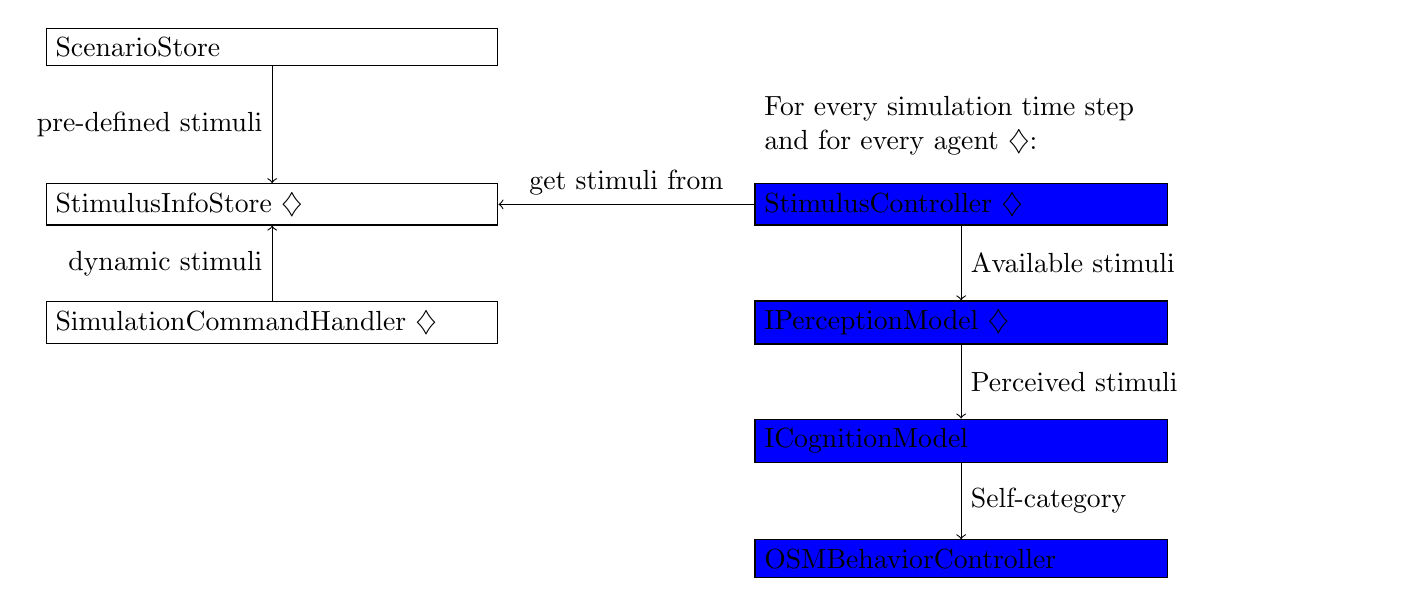
\begin{tikzpicture}
 \node[anchor=west,rectangle,draw,text width=5.5cm] (scenariostore) at (-1,3.5) {ScenarioStore};
  \node[anchor=west,rectangle,draw,text width=5.5cm] (commandhandler) at (-1,0) {SimulationCommandHandler $\diamondsuit$};
 \node[anchor=west,rectangle,draw,text width=5.5cm] (ss) at (-1,1.5) {StimulusInfoStore $\diamondsuit$};
 \node[anchor=west, text width= 5.0cm] (sc) at (8,2.5) {For every simulation time step and for every agent $\diamondsuit$:};
 \node[anchor=west,rectangle,draw,text width=5.0cm,fill=blue] (sc) at (8,1.5) {StimulusController $\diamondsuit$};
 \node[anchor=west,rectangle,draw,fill=blue,text width=5.0cm] (ip) at (8,0) {IPerceptionModel $\diamondsuit$};
 \node[anchor=west,rectangle,draw,fill=blue,text width=5.0cm] (ic) at (8,-1.5) {ICognitionModel};
 \node[rectangle,draw,anchor=west,fill=blue,text width=5.0cm] (osm) at (8,-3) {OSMBehaviorController};
 \draw[<-](ss) -- (sc) node[midway,above] {get stimuli from};
 \draw[->](sc) -- (ip) node[midway,right] {Available stimuli};
  \draw[->](ip) -- (ic) node[midway,right, text width=5.0cm] {Perceived stimuli};
   \draw[->](ic) -- (osm) node[midway,right,text width=5.0cm] {Self-category };
 \draw[->](scenariostore) -- (ss) node[midway,left] {pre-defined stimuli};
  \draw[->](commandhandler) -- (ss) node[midway,left] {dynamic stimuli};

\end{tikzpicture}
\caption[Processing dynamic stimuli in Vadere]{Processing dynamic stimuli in \textit{Vadere}. Novel or adjusted classes are marked with $\diamondsuit$. Stimuli are dynamically received over the Traffic Control Interface implemented in~\cite{schuhbaeck-2019-com}.
The adjusted \lstinline{SimulationCommandHandler} adds the stimuli to the \lstinline{StimulusInfoStore}. Since agents receive route recommendations at different times, it is necessary to address stimuli to specific agents. To achieve this, the filtering functionalities of the \lstinline{StimulusController} are extended. Also, the \lstinline{update} method of the \lstinline{IPerceptionModel} is adjusted to enable the processing of agents-specific stimuli.  }
\label{fig:processingstimuli}
\end{figure}

Due to delays, pedestrians may receive route recommendations at different times via their mobile applications. Therefore, it is mandatory that a route recommendation stimulus can be addressed to an individual agent. To achieve this, a \lstinline{SubpopulationFilter} is added to the existing \lstinline{StimulusInfo} class. The \lstinline{SubpopulationFilter} has a list attribute that contains agents ids. For agents in the list, the stimulus is forwarded to the perception layer.

Route recommendations should be only displayed in areas where they are actually needed. In real life, the mobile application would check whether information should be displayed. In the simulation, this functionality is provided by a novel spatial filter: The \lstinline{Location} attribute ensures that a stimulus is only generated for agents in a certain area. If the agent is in a certain area, the stimulus if forwarded to the perception layer.

The \lstinline{SubpopulationFilter} and the \lstinline{Location} are added to the \lstinline{StimulusInfo} as attributes. The extended class has four attributes:

\begin{itemize}
\item \lstinline{stimuli} of type \lstinline{List<Stimulus>}: route recommendations, waiting signals, bangs, ... (unchanged)
\item \lstinline{timeframe} of type \lstinline{Timeframe}: defines the time slot in which stimuli are active (unchanged)
\item \lstinline{location} of type \lstinline{Location}: defines the spatial area in which stimuli are active (novel attribute)
\item \lstinline{subpopulationFilter} of type \lstinline{SubpopulationFilter}: defines which agents have access to the stimuli (novel attribute)
\end{itemize}



The objects \lstinline{timeframe, location} and \lstinline{subpopulationFilter} are employed for filtering stimuli for space and time and address them to specific agents. The \lstinline{StimulusController} and the interface \lstinline{IPerceptionModel} are adjusted for this purpose. The filtering functionalities of the \lstinline{StimulusController} are extended to allow spatial and agent-specific filtering. Note that the original implementation only supported a time-based filtering. 

Because the provision  and the perception of a stimulus are two separate processes, I introduce two stages:
\begin{itemize}
\item First the availability of a stimulus is checked by the \lstinline{StimulusController}: Has the mobile device received a route recommendation and is this route recommendation displayed to the virtual pedestrian?
\item Second the perception is modeled at the perception layer: How is the message perceived? Are there any other stimuli?
\end{itemize}
The separation of concerns is achieved by adjusting the \lstinline{update} method of the \lstinline{IPerceptionModel} interface. Instead of using a list that contains stimuli perceived by the entire population, a map is used. Each agent has an individual list of available stimuli assigned: \lstinline{void update(HashMap<Pedestrian, List<Stimulus>> pedSpecificStimuli);}. 




\section{Module flowcontrol: novel framework for route recommendation algorithms}
\label{sec:flowcontrol}


\subsection{Scope, software architecture and requirements}
\textit{flowcontrol} is a novel Python simulation framework that I developed as part of this thesis. It is my major contribution to the \textit{CrowNet} simulation framework. The scope of \textit{flowcontrol} is to provide algorithm that generate route recommendations for crowd models.
In \textit{CrowNet}, \textit{flowcontro}l is used in combination with the \textit{Vadere} simulator. 
%
\textit{flowcontrol} has a modular architecture and follows a model view controller pattern, see Fig.~\ref{fig:mvcflow}. 


\begin{figure}[hbt!]
\includegraphics[width=\textwidth]{./crownet/flowcontrol_MVC.pdf} 
\caption[flowcontrol: packages and important classes of the Python  framework ]{Architecture of the novel simulation framework \textit{flowcontrol}. The scope of \textit{flowcontrol} is to provide route recommendations for pedestrian dynamics simulators, such as \textit{Vadere}.  Route recommendation algorithms, time stepping procedures and methods for mapping sensor data are implemented in the \lstinline{strategy} package (`Model'). The data exchange with other simulators is handled in \lstinline{crownetcontrol/traci} (`Controller'). \textit{flowcontrol} uses the graphical user interface of the crowd simulator: The \lstinline{dataprocessor} package (`View') provides additional data processors. }
\label{fig:mvcflow}
\end{figure}


The \lstinline{strategy} package (`Model') contains the core elements for generating route recommendations. It contains several sub-packages, see again Fig.~\ref{fig:mvcflow}. 
The \lstinline{controller} sub-package contains the route recommendation algorithms. The \lstinline{timestepping} sub-package contains methods to control the time between two route recommendations. The sub-package \lstinline{controlaction} provides representations for route recommendations. For example, the \textit{Vadere} simulator requires that a route recommendation is a \lstinline{StimulusInfo} object in JSON format. To couple \textit{flowcontrol} with another pedestrian dynamics simulator, one simply implements the simulator-specific representation of a route recommendation.


The package \lstinline{crownetcontrol/traci} (`Controller') manages the transfer of route recommendations over the Traffic Control Interface. If the complete crowd guidance system should be simulated, the recommendation is sent to \textit{OMNeT++}. \textit{OMNeT++} simulates the transmission of the route recommendation in the mobile network. When the packet is received, the route recommendation is forwarded to \textit{Vadere}. When the network simulation is not needed, \textit{flowcontrol} sends the route recommendation directly to \textit{Vadere}. Depending on the simulator combination, \textit{flowcontrol} is either the client or the server, see again Fig.~\ref{fig:configurationCrownet} in Section~\ref{sec:crownetutils}. 

 
As most pedestrian simulators \textit{Vadere} provides a graphical user interface and visualization tools which is why \textit{flowcontrol} does not provide a user interface. The processors and export functionalities in the  \lstinline{dataprocessor} package (`View') only serve to verify the results. 

For the development of \textit{flowcontrol}, I adhere to the principles of software development: I use code quality measures (see Section~\ref{sec:requirementglobal}) and define requirements, see Tab.~\ref{tab:requirementsflowcontrol}. \textit{flowcontro}l has an own continuous integration pipeline that is triggered with every commit. Unit tests verify the correct implementation of methods. Integration tests ensure that the simulator coupling works.




\begin{table}[hbt!]
\begin{tabular}{|p{7cm}|p{7cm}|}
\hline
\textbf{Requirement} & \textbf{Design decisions}  \\
\hline 
Route recommendation algorithms for crowds must be provided that can be transferred to arbitrary scenarios; adding algorithms should be easy. & Provide algorithms that can be transferred to arbitrary scenarios; establish a reusable software structure by using suitable interfaces and a strategy pattern (see Section~\ref{sec:routerecommendationalgorithms}).  \\ \hline
 It must be possible to control the time between two evaluations of the route recommendation algorithm (time interval). & Separate the time stepping procedure from the logic of the algorithm and provide time stepping procedures (see Section~\ref{sec:timestepping}). \\ \hline
It should be possible to use density information from the decentralized density maps application (Section~\ref{sec:novelapplication}) as input for the route recommendation algorithm. & Implement a procedure that extracts the necessary density information from the application data (see Section~\ref{sec:mappingproc}).  \\
\hline
\end{tabular} 
\caption[Requirements on the novel flowcontrol simulator.]{Main requirements for the novel \textit{flowcontrol} simulator. The design decisions (right) describe how the requirements for the simulator (left) are implemented.  }
\label{tab:requirementsflowcontrol}
\end{table}




\FloatBarrier


\subsection{Route recommendation algorithms: the logic of guidance}
\label{sec:routerecommendationalgorithms}
The redirection logic of the route recommendation algorithm is implemented in the \lstinline{strategy} module. To enable developers to easily extend the simulation framework, a strategy software design pattern is used. With this, new algorithms can be simply added by inheriting from the abstract class \lstinline{RouteRecommendationAlgorithm}, see Fig.~\ref{fig:routerecommalg}. 
The static helper method \lstinline{get_controller_from_args} creates and initializes an object of the type \lstinline{RouteRecommendationAlgorithm} defined in \lstinline{run_script.py} (\lstinline{--ctrl.controller-type}). The separation of algorithm logic and object initialization allows to extend the package easily which increases the re-usability and sustainability of the software. 


As I have outlined in the state of the art, several algorithms have been proposed for guiding crowds (see Section~\ref{sec:modelalg}). However, these are neither transferable to arbitrary scenarios, nor have they been tested under realistic conditions. Therefore I develop algorithms myself and implement them in the \lstinline{strategy} package. 

I suggest and implement the following algorithms:
\begin{itemize}
\item \lstinline{AlternateTargerAlgorithm}: alternates the routes sequentially.
\item \lstinline{AvoidCongestionAlgoritm}: recommends an alternative route whenever the density on the direct route is higher than on the alternative route.
\item \lstinline{MinimalDensityAlgorithm}: recommends the route where the density is the lowest. If there are only two routes, the algorithm is identical to \lstinline{AvoidCongestionAlgorithm}.
\end{itemize}


\begin{figure}[hbt!]
\includegraphics[width=\textwidth]{./crownet/flowcontrol_UML_guiding_strategy.pdf} 
\caption{Important classes for the implementation of route recommendation algorithms in the \lstinline{strategy} module. The core of the module is the abstract class \lstinline{RouteRecommendationAlgorithm}. The logic of a route recommendation algorithm is implemented in the \lstinline{get_next_target()} method of the respective child class.  }
\label{fig:routerecommalg}
\end{figure}



\subsection{Time stepping procedure }

\label{sec:timestepping} 

A core functionality of a dynamic crowd guidance system is the scheduling of route recommendations. In \textit{flowcontrol} this functionality is implemented in the \lstinline{timestepping} module. \textit{flowcontrol} offers different types of time stepping procedures that trigger the generation of route recommendation at regular or irregular time intervals, see Fig.~\ref{fig:timestepper}. 




\begin{figure}[hbt!]
\includegraphics[width=\textwidth]{./crownet/flowcontrol_UML_timestepping.pdf} 
\caption[flowcontrol: Implementation of the time stepping]{
Time stepping procedure. The abstract class \lstinline{TimeStepper} controls the time in between two route recommendations. The time interval can be either fixed (\lstinline{FixedTimeStepper}) or dynamically adjusted during the simulation (\lstinline{AdaptiveTimeStepper}). For the latter, a \lstinline{StepSizeAlgorithm} is required that computes when the route recommendation algorithm should be evaluated next. }
\label{fig:timestepper}
\end{figure}

With a static stepping procedure, the time between two route recommendations is always the same. A dynamic stepping procedure adjusts the time between two route recommendations dynamically. A dynamic adjustment may help to reduce the number of redirection measures. This might be particularly helpful when the number of pedestrians changes dynamically over time: At a low arrival rate few redirection measures may be needed (large time interval) to dissolve congestion. At a high arrival rate (small time interval), pedestrians may need to be redirected more often. Therefore, the \lstinline{StepSizeAlgorithm} interface is introduced. Its core method is the abstract method \lstinline{get_next_time_step_size()} that has to be implemented by the child classes. 

\subsection{Extracting density information from density maps}
\label{sec:mappingproc}

Some route recommendation algorithms require density measurements. Densities are measured in areas where the maximum densities occur. I want to measure densities based on direct communication technology which is why I propose to use the decentralized density map application~\cite{schuhbaeck-2023-com}. However, a measurement area does not always correspond to a specific cell of the map, see Fig.~\ref{fig:mappingproblem}. 


\begin{figure}[H]
\centering
\includegraphics[width=0.9\textwidth]{./crownet/mappingalg.pdf} 
\caption[]{Mapping of density data. Since the measurement area is does not correspond to one cell of the density map application~\cite{schuhbaeck-2023-com}, a mapping is required. If obstacles cover parts of the cell, the reference area is small which leads to high densities (right). }
\label{fig:mappingproblem}
\end{figure}


The \lstinline{sensor} package provides a mapping procedure that computes the average density from cell-based data. The averaging procedure is implemented in the \lstinline{DensityMapper} that has information about the cell layout, the measurement areas and the obstacles, see Fig.~\ref{fig:densitymap}.  Since the density map application does not consider obstacles, densities could be locally underestimated which is not acceptable for crowd management applications. A simple correction procedure is implemented: The percentage of available space is determined for each cell. Then the density values are divided by the percentage values, given that a cell is not fully occupied by an obstacle.



\begin{figure}[H]
\includegraphics[width=\textwidth, trim=0.2cm 8.6cm 0.2cm 0.2cm, clip]{./crownet/flowcontrol_UML_sensor.pdf} 
\caption[Density estimation: implementation of a mapping approach ]{Important classes for the density estimation. The \lstinline{DensityMapper} has information about the measurement area (position, size) and the cell-grid (cell size, cell position). The \lstinline{DensityMapper}  estimates the crowd density in a measurement area from a density map~\cite{schuhbaeck-2023-com}.  }
\label{fig:densitymap}
\end{figure}










\section{Summary}

With \textit{CrowNet}, I created a new open-source framework to simulate a crowd guidance system where crowds are sensed and redirected using direct communication technology. First, I modeled a crowd guidance system composed of a crowd, a controller containing the route recommendation algorithm, a mobile application for sensing the crowd, and a mobile application for communicating route recommendations. Based on the model structure, I designed a modular software architecture. For the implementation, I defined functional and non-functional requirements and made design decisions to be realized in the corresponding modules. In addition, quality measures were defined to ensure software quality and sustainability. A continuous integration and deployment pipeline was introduced to test the source code during the development process. The core functionalities of the software were then implemented in the five main modules.

The \textit{crownetutils} module provides implementations for coupling models and simulators. An explicit update procedure was proposed and implemented, interpolating agent positions in the mobile communication simulation. To separate the inter-process communication of simulators from parallel executions and from the host system, the coupled simulation are executed in a containerized fashion, employing Docker networks. The state exchange between simulators is realized via the Traffic Control Interface. Several simulator couplings have been implemented for the simulation of the entire crowd system and for isolated subsystems. 

The \textit{SUQ-controller} enables to conduct parameter studies with coupled simulations. The module is based on the existing Python package \textit{SUQ-controller}. New process calls were added in order to be able to run coupled simulations. The definition of parameter combinations has also been extended. Parameters can now be changed in various simulator-specific config files. To ensure that only Docker containers communicate that refer to a specific parameter combination, a naming convention for the containers has been introduced.

The \textit{OMNeT++} module enables the simulation of direct communication. Existing simulators were employed as model libraries for the lower layers of the network. To sense crowds, a novel method based on LTE sidelink communication was implemented: the decentralized pedestrian density map application. Two further mobile applications were implemented to disseminate route recommendations, which differ in their static or dynamic information content.

The \textit{Vadere} module provides crowd models. The analysis of the state-of-the-art simulator showed that several extensions were required for the integration of \textit{Vadere} into \textit{CrowNet}: First, I generalized the stimulus definition and the processing of the stimuli in \textit{Vadere}'s psychology layer to enable dynamically generated route recommendations to be processed. Second, I introduced an interface for modeling probabilistic behavior in the cognition layer to enable probabilistic route choice. Third, I parameterized the psychology layer to permit parameter studies with behavioral models. With these extensions, route recommendations can be dynamically processed in \textit{Vadere}'s psychology layer. 

The module \textit{flowcontrol} has been developed for the provision of route recommendations. For this novel Python framework I first defined requirements from which I derived design decisions. Since state-of-the-art route recommendation algorithms did not fulfill my requirements, I proposed novel algorithms and implemented them. To control the time interval between two route recommendations, a generic time-stepping procedure has been implemented. To handle sensor data, a method was implemented that maps cell-based density values, provided by the density map application, to measurement areas. The \textit{flowcontrol} framework can be combined with other crowd simulators by implementing appropriate interfaces.


In the following chapter, I will use the \textit{CrowNet} software as a simulation tool to investigate my research question.